\begin{figure}
    \centering

    \tikzset{every picture/.style={line width=0.75pt}} %set default line width to 0.75pt        

    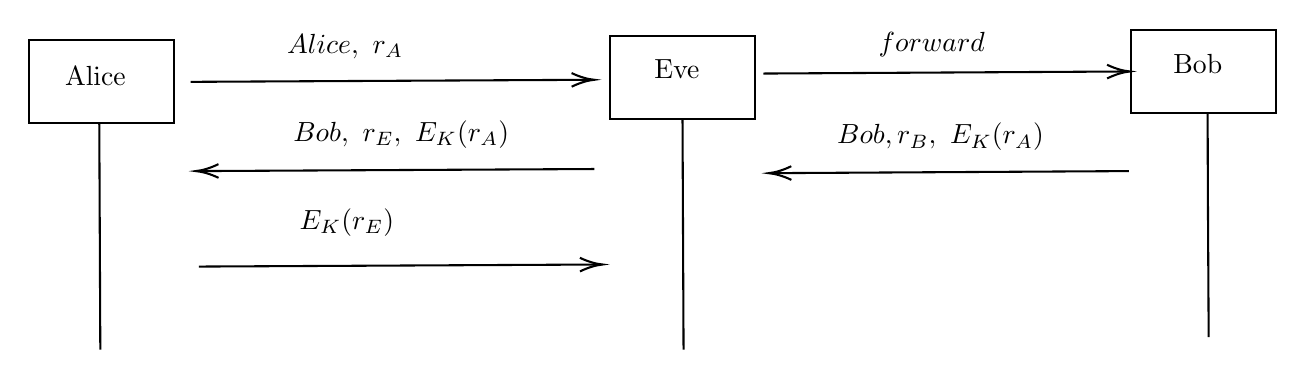
\begin{tikzpicture}[x=0.75pt,y=0.75pt,yscale=-1,xscale=1]
    %uncomment if require: \path (0,230); %set diagram left start at 0, and has height of 230

    %Shape: Rectangle [id:dp1743019806713867] 
    \draw   (32,32) -- (102,32) -- (102,72) -- (32,72) -- cycle ;

    %Shape: Rectangle [id:dp6293669652442805] 
    \draw   (563,27) -- (633,27) -- (633,67) -- (563,67) -- cycle ;

    %Shape: Rectangle [id:dp9205463275779588] 
    \draw   (312,30) -- (382,30) -- (382,70) -- (312,70) -- cycle ;

    %Straight Lines [id:da9822614621505796] 
    \draw    (110,52) -- (302.5,51.01) ;
    \draw [shift={(304.5,51)}, rotate = 179.71] [color={rgb, 255:red, 0; green, 0; blue, 0 }  ][line width=0.75]    (10.93,-3.29) .. controls (6.95,-1.4) and (3.31,-0.3) .. (0,0) .. controls (3.31,0.3) and (6.95,1.4) .. (10.93,3.29)   ;
    %Straight Lines [id:da8180326777766349] 
    \draw    (66,72) -- (66.5,181) ;
    %Straight Lines [id:da7527020702065276] 
    \draw    (347,70) -- (347.5,181) ;
    %Straight Lines [id:da7872518105548856] 
    \draw    (600,67) -- (600.1,102) -- (600.5,175) ;
    %Straight Lines [id:da6977144240055365] 
    \draw    (386,48) -- (560.5,47.01) ;
    \draw [shift={(562.5,47)}, rotate = 179.68] [color={rgb, 255:red, 0; green, 0; blue, 0 }  ][line width=0.75]    (10.93,-3.29) .. controls (6.95,-1.4) and (3.31,-0.3) .. (0,0) .. controls (3.31,0.3) and (6.95,1.4) .. (10.93,3.29)   ;
    %Straight Lines [id:da6481231910605018] 
    \draw    (562,95) -- (390.5,95.99) ;
    \draw [shift={(388.5,96)}, rotate = 359.67] [color={rgb, 255:red, 0; green, 0; blue, 0 }  ][line width=0.75]    (10.93,-3.29) .. controls (6.95,-1.4) and (3.31,-0.3) .. (0,0) .. controls (3.31,0.3) and (6.95,1.4) .. (10.93,3.29)   ;
    %Straight Lines [id:da28842039284308707] 
    \draw    (304.5,94) -- (114.5,94.99) ;
    \draw [shift={(112.5,95)}, rotate = 359.7] [color={rgb, 255:red, 0; green, 0; blue, 0 }  ][line width=0.75]    (10.93,-3.29) .. controls (6.95,-1.4) and (3.31,-0.3) .. (0,0) .. controls (3.31,0.3) and (6.95,1.4) .. (10.93,3.29)   ;
    %Straight Lines [id:da5471284771409243] 
    \draw    (114,141) -- (306.5,140.01) ;
    \draw [shift={(308.5,140)}, rotate = 179.71] [color={rgb, 255:red, 0; green, 0; blue, 0 }  ][line width=0.75]    (10.93,-3.29) .. controls (6.95,-1.4) and (3.31,-0.3) .. (0,0) .. controls (3.31,0.3) and (6.95,1.4) .. (10.93,3.29)   ;

    % Text Node
    \draw (48,43) node [anchor=north west][inner sep=0.75pt]   [align=left] {Alice};
    % Text Node
    \draw (582,37) node [anchor=north west][inner sep=0.75pt]   [align=left] {Bob};
    % Text Node
    \draw (332,40) node [anchor=north west][inner sep=0.75pt]   [align=left] {Eve};
    % Text Node
    \draw (155,27.4) node [anchor=north west][inner sep=0.75pt]    {$Alice,\ r_{A}$};
    % Text Node
    \draw (440,26.4) node [anchor=north west][inner sep=0.75pt]    {$forward$};
    % Text Node
    \draw (420,70.4) node [anchor=north west][inner sep=0.75pt]    {$Bob,r_{B} ,\ E_{K}( r_{A})$};
    % Text Node
    \draw (158,69.4) node [anchor=north west][inner sep=0.75pt]    {$Bob,\ r_{E} ,\ E_{K}( r_{A})$};
    % Text Node
    \draw (161,111.4) node [anchor=north west][inner sep=0.75pt]    {$E_{K}( r_{E})$};


    \end{tikzpicture}


    \caption{Forward and change nounce attack}\label{fig:forward_attack}
\end{figure}

The second attack (\autoref{fig:reflec_attack}) is based on the reflection in which the same challenge-respone
protocol is used by each side to authenticate. In this case, receiving the random
number \(r_A\), Eve opens another connection to Alice and sends the \(r_A\) as 
the challenge. Responding to the challenge, Alice sends back the encryption of
\(r_A\), \(E_K(r_A)\) using secret key \emph{K}, so Eve may use the \(E_K(r_A)\)
as the response for the orginal connection.

\begin{figure}
    \centering

    \tikzset{every picture/.style={line width=0.75pt}} %set default line width to 0.75pt        

    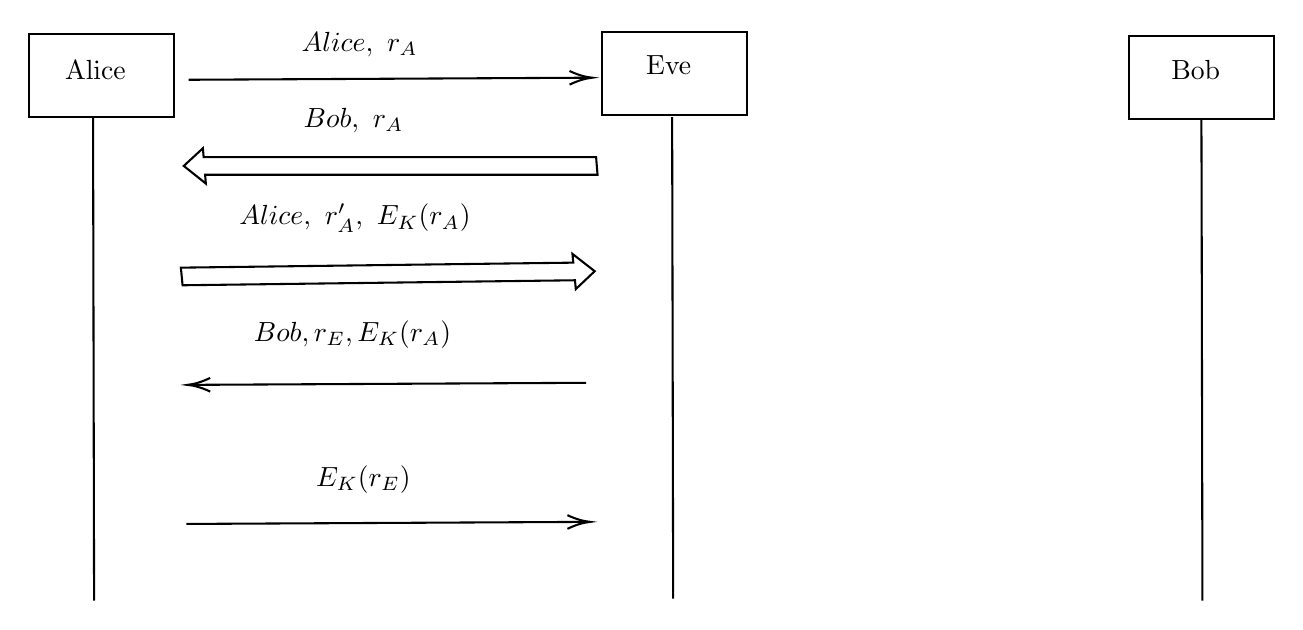
\begin{tikzpicture}[x=0.75pt,y=0.75pt,yscale=-1,xscale=1]
    %uncomment if require: \path (0,304); %set diagram left start at 0, and has height of 304

    %Shape: Rectangle [id:dp4307414355730742] 
    \draw   (38,14) -- (108,14) -- (108,54) -- (38,54) -- cycle ;

    %Straight Lines [id:da6699282610873214] 
    \draw    (69,54) -- (69.5,287) ;
    %Shape: Rectangle [id:dp14413221032472534] 
    \draw   (314,13) -- (384,13) -- (384,53) -- (314,53) -- cycle ;

    %Straight Lines [id:da2594747996425629] 
    \draw    (348,54) -- (348.5,286) ;
    %Shape: Rectangle [id:dp6795112051058219] 
    \draw   (568,15) -- (638,15) -- (638,55) -- (568,55) -- cycle ;

    %Straight Lines [id:da2700892625832104] 
    \draw    (603,55) -- (603.1,90) -- (603.5,287) ;
    %Straight Lines [id:da6280779364864771] 
    \draw    (115,36) -- (307.5,35.01) ;
    \draw [shift={(309.5,35)}, rotate = 179.71] [color={rgb, 255:red, 0; green, 0; blue, 0 }  ][line width=0.75]    (10.93,-3.29) .. controls (6.95,-1.4) and (3.31,-0.3) .. (0,0) .. controls (3.31,0.3) and (6.95,1.4) .. (10.93,3.29)   ;
    %Left Arrow [id:dp4487245190088919] 
    \draw   (112.71,77.5) -- (121.93,69) -- (122.28,73.25) -- (311.36,73.25) -- (312.06,81.75) -- (122.99,81.75) -- (123.34,86) -- cycle ;
    %Left Arrow [id:dp43694862025128633] 
    \draw   (310.7,128.23) -- (301.59,136.85) -- (301.18,132.6) -- (112.13,135.01) -- (111.31,126.52) -- (300.37,124.11) -- (299.96,119.87) -- cycle ;
    %Straight Lines [id:da6742120284938153] 
    \draw    (306.5,182) -- (116.5,182.99) ;
    \draw [shift={(114.5,183)}, rotate = 359.7] [color={rgb, 255:red, 0; green, 0; blue, 0 }  ][line width=0.75]    (10.93,-3.29) .. controls (6.95,-1.4) and (3.31,-0.3) .. (0,0) .. controls (3.31,0.3) and (6.95,1.4) .. (10.93,3.29)   ;
    %Straight Lines [id:da800462964668085] 
    \draw    (114,250) -- (306.5,249.01) ;
    \draw [shift={(308.5,249)}, rotate = 179.71] [color={rgb, 255:red, 0; green, 0; blue, 0 }  ][line width=0.75]    (10.93,-3.29) .. controls (6.95,-1.4) and (3.31,-0.3) .. (0,0) .. controls (3.31,0.3) and (6.95,1.4) .. (10.93,3.29)   ;

    % Text Node
    \draw (54,25) node [anchor=north west][inner sep=0.75pt]   [align=left] {Alice};
    % Text Node
    \draw (334,23) node [anchor=north west][inner sep=0.75pt]   [align=left] {Eve};
    % Text Node
    \draw (587,25) node [anchor=north west][inner sep=0.75pt]   [align=left] {Bob};
    % Text Node
    \draw (168,11.4) node [anchor=north west][inner sep=0.75pt]    {$Alice,\ r_{A}$};
    % Text Node
    \draw (169,48.4) node [anchor=north west][inner sep=0.75pt]    {$Bob,\ r_{A}$};
    % Text Node
    \draw (138,94.4) node [anchor=north west][inner sep=0.75pt]    {$Alice,\ r_{A} ',\ E_{K}( r_{A})$};
    % Text Node
    \draw (145,150.4) node [anchor=north west][inner sep=0.75pt]    {$Bob,r_{E} ,E_{K}( r_{A})$};
    % Text Node
    \draw (175,220.4) node [anchor=north west][inner sep=0.75pt]    {$E_{K}( r_{E})$};


    \end{tikzpicture}


    \caption{Reflection attack}\label{fig:reflec_attack}
\end{figure}